\presec \section{Computing the Optimal k} \postsec \label{sec:optimalk}
%
Traditionally, the optimal number of hash functions is derived through finding the extrema of the asymptotic formula of $f_{bloom}$ given in Eq. \ref{fBloom} as follows:
%
\begin{equation}
\label{eq:kopt}
k^*_{bloom}=\frac{m}{n}\ln 2
\end{equation}
%
However, as we have discussed, the underlying formula for FP probability is not fully correct. 
%
In this section, we first present the important theorems that correlate information entropy and the false positive rate of Bloom filters.
%
Then we propose a method of deriving the optimal value of $k$ by minimizing the FP probability given the value of BF size $m$ and number of inserted elements $n$.

\presub \subsection{Information Entropy Basis} \postsub
%
\noindent\textbf{Information Entropy}: In information theory, \textit{information entropy} is used to measure the uncertainty of a random variable.
%
In this paper, we use \textit{Shannon entropy} \cite{shannon}, which measures the value of the information contained in a variable. 
%
Entropy is typically measured in bits, nats, or bans \cite{entropy}. 
%
For a variable with $s$ events with the probabilities of $p_1$, $p_2$, ..., $p_s$. 
%
The information entropy $E$ is defined as:
%
\begin{equation}
 E=\sum_{i=1}^{s}p_i  log_2 \dfrac{1}{p_i}
\label{equ:entropy}
\end{equation}

\noindent\textbf{Property of Information Entropy:}
%
For any variable or message, if its information entropy is not at the maximum, it can be compressed without information losses. 
%
For a random variable, the larger the uncertainty is, the bigger the information entropy is.
%
Suppose an $m$-bit string variable is compressed to $m'$-bit string variable, the entropy becomes $E'$ from $E$. 
%
Then we have $mE=m'E'$.
%
According to the information entropy formula (Eq. \ref{equ:entropy}), we can obtain the information entropy $E$ of the $m$-bit variable of a BF as follows, where $p'$ is defined in Equation \ref{p'form}.

\begin{equation}
E=-\left(p'\log_2 p' +(1-p')\log_2(1-p')\right)
\label{equ:entropyBF}
\end{equation}

We illustrate the relationship between entropy $E$ and $p'$ in Figure \ref{fig:entropy}. 
%
We can observe that the entropy of an $m$-bit sequence reaches the maximum when the probability that each bit in the BF is 1 (or 0) is $50\%$.

\begin{figure}[htbp]
\centering
\prefig
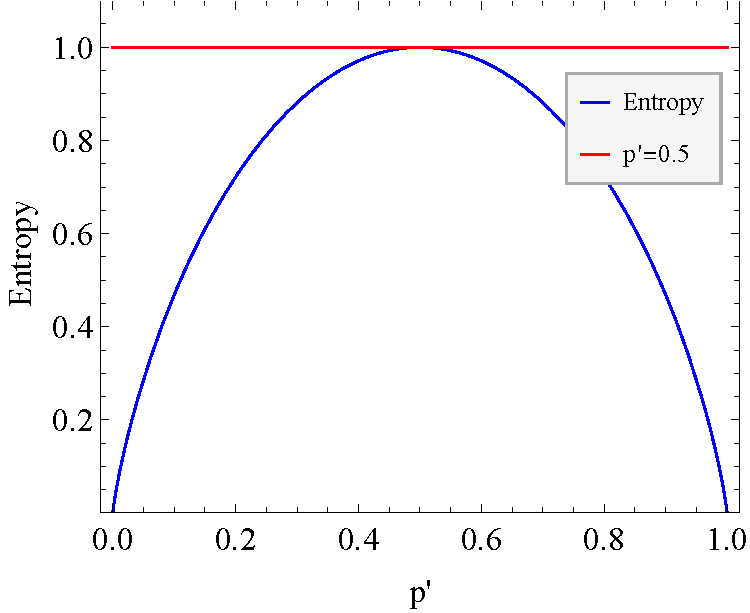
\includegraphics[width=\figwidth]{entropy}
\postfig\precaption
\caption{Information entropy of a BF}
\postcaption
\label{fig:entropy}
\end{figure}

\presub \subsection{Relation Between False Positive Probability and Information Entropy} \postsub
%
We now show the relation between the false positive probability and information entropy. 
%
We first present a lemma and some definitions.

\noindent\textbf{Lemma I:} Given a BF, suppose $n$ and $k$ keep unchanged, when $m$ becomes larger, the FP probability gets smaller.

\begin{proof}
When $n$ and $k$ are fixed, for larger $m$, the probability of each bit being 1 in the BF becomes smaller, \ie, $p'$ becomes smaller; thus, the FP probability gets smaller.
\end{proof}

%%
\noindent\textbf{Definition I:} \textit{Bloom filter variable.} The false positive rate of Bloom filters is determined by $m$, $n$, and $k$. For different $n$ elements, the $m$-bit string varies. Thus, when the values of $m$, $n$, $k$ are given, the $m$-bit string is a \textit{random variable}. When the $n$ elements are given, the $m$-bit string is a random variable instance. Therefore, when the values of $m$, $n$, $k$ are given, we call it a Bloom Filter Variable (BFR). Since it is a random variable, we can compute its information entropy.

\noindent\textbf{Definition II:} \textit{Equivalent Bloom filter variables.} Given two Bloom filters variables $v_1$ and $v_2$, for the same $n$ elements, there are a pair of BFR instances. Given a set with $n$ elements, if these pairs of BFR instances always report the same result: true or false for any input element, we say $v_1$ and $v_2$ are equivalent.

\noindent\textbf{Theorem I:} Given a Bloom filter \textit{variable} $v_1$ with parameters $m$, $n$, and $k$, if its information entropy is not at the maximum, there must exist a smaller equivalent Bloom filter variable $v_2$ with parameters $m'$, $n$ and $k$, where $m'<m$.

\begin{proof}
For $v_1$, the parameters are $m$, $n$, $k$. 
%
Suppose its $k$ hash functions are $h_1(\cdot), h_2(\cdot), \ldots, h_k(\cdot)$.
%
Since the assumption is that the information entropy of $v_1$ is not at the maximum, according to the property of information entropy, $v_1$ can be compressed \textit{without information loss}. 
%
After compression, suppose the new random variable has a length of $m' (m' < m)$, we name it $v_2$.
%
Note that during the compression, the information value $m*E$ keeps unchanged, while $E's$ maximum value is 1; thus, the length of the compressed message has a minimum value.
%
Here $v_1$ and $v_2$ are two variables consisting of bits, and we can treat them as two integer variables. 
%
We use $In(v_1)$ and  $In(v_2)$ to represent the integer value of $v_1$ and $v_2$.
%
Furthermore, we use $|In(v_1)|$ represents the length of $v_1$, then we have  $|In(v_1)|=m$, $|In(v_2)|=m'$.
%
Because we compress $v_1$ and get $v_2$, this can be regarded as a function $g(\cdot)$. 
%
In other words, $g(In(v_1))=In(v_2)$. 
%
We can also obtain $v_1$ by equation $In(v_1)=g^{-1}(In(v_2))$.

At this stage, we consider the new Bloom filter variable $v_2$, the parameters are $m'$, $n$, and $k$.
%
Note that we use $k$ \texttt{different} hash functions, and the $k$ hash functions are
%
\begin{equation}
\begin{aligned}
&g^{-1}(In(v_2))\ll h_1(y) \gg (|g^{-1}(In(v_2))|-h_1(y)-1), \\
&g^{-1}(In(v_2))\ll h_2(y) \gg (|g^{-1}(In(v_2))|-h_2(y)-1), \\
& \ldots \\
&g^{-1}(In(v_2))\ll h_k(y) \gg (|g^{-1}(In(v_2))|-h_k(y)-1)
\end{aligned}
\label{equ:g(k)}
\end{equation}
%
Where `$\ll$' means left shift and `$\gg$' means right shift.

Given an input element $y$, we can compute the above $k$ values only using $v_2$ and $h_i(\cdot)$ without $v_1$.
%
Then we need to prove that for any incoming element $y$, $v_2$ reports the same $k$-bit value.
%
With formula \ref{equ:g(k)}, we use equation $v_1=g^{-1}(In(v_2))$ and $m=|g^{-1}(In(v_2))|$.
%
These $k$ hash functions are simplified as
%
\begin{equation}
\begin{aligned}
&v_1\ll h_1(y) \gg (m-h_1(y)-1), \\
&v_1\ll h_2(y) \gg (m-h_2(y)-1), \\
& \ldots \\
&v_1\ll h_k(y) \gg (m-h_k(y)-1)
\end{aligned}
\label{equ:g(k):simple}
\end{equation}
%
Here $1\leqslant i\leqslant k$ and $0\leqslant h_i(y)\leqslant m-1$.
%
Here $v_1\ll h_i(y) \gg (m-h_i(y)-1)$ actually means the value of $h_i(y)$-th bit of $v_1$.
%
This is the same as the $k$ hash functions as $v_1$. 
%
Therefore, $v_1$ and $v_2$ are equivalent.
\end{proof}

\noindent\textbf{Theorem II:} Given a Bloom filter variable,  \textit{if and only if} its information entropy is at the maximum, its FP probability is at the minimum.

\begin{proof}
%
First, we prove that if the FP probability is at the minimum, then its information entropy must be at the maximum. 
%
Given a Bloom filter variable $v_1$ with parameters $m$, $n$, $k$. 
%
Since the assumption is that the information entropy of $v_1$ is not at the maximum, according to Theorem I, there exists a smaller Bloom filter variable $v_2$ with parameters $m'$, $n$, $k$. 
%
Since $v_2$ and $v_1$ are equivalent, their FP probabilities are the same, we name it $f$.
%
At this stage, we enlarge the size of $v_2$ a little from $m'$ to $m''$, where $m'<m''<m$. 
%
According to Lemma I, we know the FP probability of $v_2$ becomes smaller than $f$. 
%
This means that for $v_1$, there exists a BF variable with a smaller size and a smaller FP probability.
%
Therefore, the FP probability of $v_1$ is not at the minimum.
%
This means that if its information entropy is not at the maximum, then the FP probability is definitely not at the minimum. 
%
The contrapositive is that if the FP probability is at the minimum, then its information entropy must be at the maximum.

%%
Second, we prove that if its information entropy is at the maximum, the FP probability is at the minimum.
%
Given a Bloom filter variable $v_1$ with parameters $m$, $n$, $k$. 
%
Since the assumption is that the FP probability of $v_1$ is not at the maximum, there exists an optimal Bloom filter variable $v_0$ with parameters $m$, $n$, $k'$, where $k'\neq k$. 
%
According to $\leftarrow$, the information entropy of $v_0$ is at the maximum. 
%
According to Eq. \ref{equ:entropyBF} and Figure \ref{fig:entropy}, the $p'$ of $v_0$ is 0.5 whereas the $p'$ of $v_1$ is not because they have different value of $k$. 
%
Therefore, the information entropy of BF$_1$ is not at the maximum.
%
This means if the FP probability is not at the minimum, its information entropy must be not at the maximum. 
%
The contrapositive is that if its information entropy is at the maximum, the FP probability is at the minimum.
\end{proof}

\presub \subsection{Computing the Optimal k} \postsub
\label{optk}
%
According to Theorem II, when the information entropy of the Bloom filter variable is at the maximum, the FP probability is at the minimum.
%
Recalling the definition of $p'$ in Eq. \ref{p'form}, one can use this interpretation to find $k^*$, \ie, the optimal number of hash functions. 
%
From Figure \ref{fig:entropy}, we know that when $p'$ is 0.5, $E$ reaches the maximum value 1. By setting the value of $p'$ to 0.5, we have
%
\begin{equation}
p'=\left(1-\frac{1}{m}\right)^{k^* n}=0.5
\label{equ:p=0.5}
\end{equation}
%
Further, we have:
\begin{equation}
\label{equ:mykform}
k^*=-\dfrac{\ln 2}{n} / \ln\left(1-\dfrac{1}{m}\right)
\end{equation}
%
This formula is very close to the formula of $k^*$ obtained by Bloom. 
%
When $x$ is very small, $\ln(1+x)\approx x$, and therefore $-1/\ln(1-\dfrac{1}{m}) \approx m$, resulting the same term as in Eq. \ref{eq:kopt}.

\noindent\textbf{Theorem III:} Given any BF variable, when $m$ and $n$ are fixed, the FP probability $f$ is a function of $k$, we represent it $f(k)$. Then $f(k)$ is a \textit{convex function}, which has only one minimum value.

\begin{proof}
Given a Bloom filter variable $v_1$ with parameters $m$, $n$, $k_1$, its entropy is $E_1$.
%
Given another Bloom filter variable $v_2$ with parameters $m$, $n$, $k_2$, its entropy is $E_2$.
%
(1) For any $k_1<k_2\leqslant k^*$, according to Eq. \ref{p'form}, Eq. \ref{equ:entropyBF} and Figure \ref{fig:entropy}, we known $p'_1<p'_2\leqslant 0.5$.
%
We compress $v_1$ to $v_3$ with parameters $m_3$, $n$, $k_1$. 
%
To make $v_3$'s entropy equal to $E_2$, $m_3$ should be $mE_1/E_2$. 
%
In this case, the entropy of $v_3$ is equal to that of $v_2$. 
%
When the entropy of BF variables is less than 0.5, the same entropy leads to the same $p'$. 
%
In other words, $p'_3=p'_2$. 
%
Because $v_2$ has more hash functions ($k_2>k_1$), the FP probability of $v_2$ is smaller than that of $v_3$. 
%
While $v_3$ and $v_1$ have the same FP probability, therefore, the FP probability of $v_2$ is smaller than that of $v_1$.
%
In other words, for any $k (k<k^*)$ increasing, the FP probability of BFs decreases.
%
(2) For any $k^*\leqslant k_1<k_2$, according to Eq. \ref{p'form}, Eq. \ref{equ:entropyBF} and Figure \ref{fig:entropy}, we known $p'_1>p'_2\geqslant 0.5$.
%
Using the similar derivation, we can derive that the FP probability of $v_2$ is larger than that of $v_1$.
%
According to the above two cases, we know that given any BF variable, when $m$ and $n$ are fixed, the FP probability $f$ is a function of $k$, we represent it $f(k)$.  
%
So $f(k)$ is a \textit{convex function}.
\end{proof}